\section*{7. Recursive Observation and Entanglement Symmetry}
\label{sec:recursive-observation}

\subsection*{7.1 Observation as a Physical Process}

In the recursive cosmological framework, observation is not an external act—it is a fundamental, endogenous process. Each cycle \( n \) serves as an observer of the next cycle \( n+1 \), transferring structure, memory, and phase information through the transition kernel \( K(\phi, \phi') \). This implements a recursive form of Quantum Darwinism~\cite{zurek_quantum_2009,zurek_environment-induced_2003}: only systems that maintain coherence across the boundary propagate forward.

We define observation as the \textit{intersection of signal with structure}—the event wherein retained coherence modulates the configuration of the next cycle. This generalizes the act of measurement beyond consciousness, aligning with the information-theoretic formulations of~\cite{tegmark_consciousness_2015}.
\begin{figure}[H]
\centering
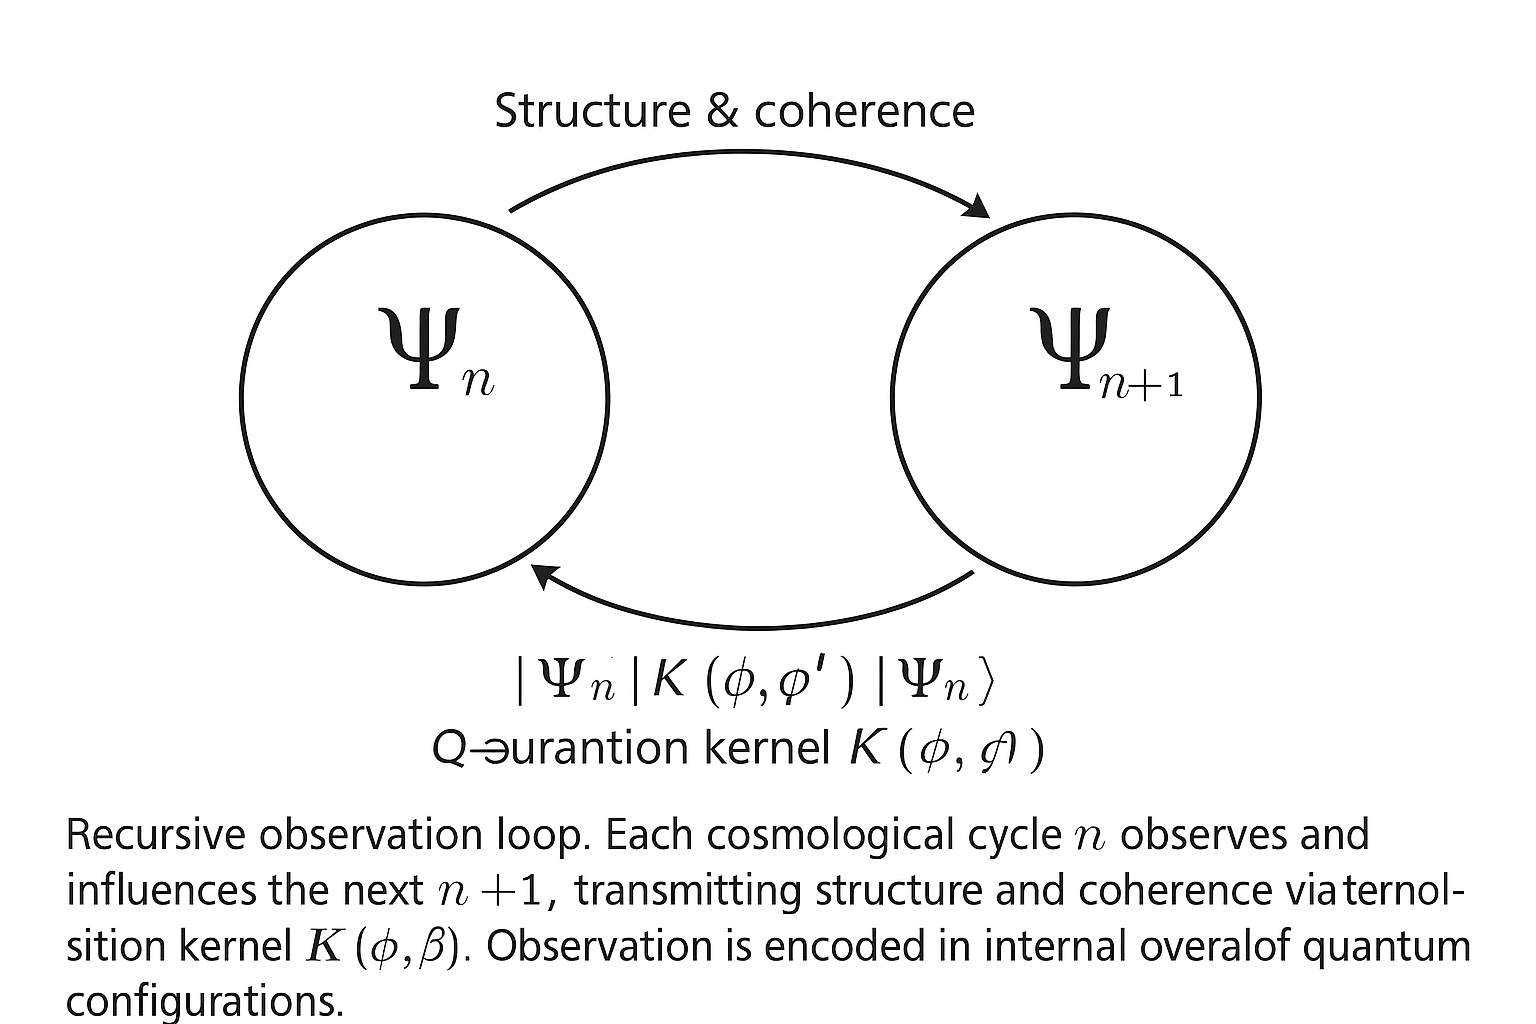
\includegraphics[width=0.75\textwidth]{figures/recursive_observation_loop.png}
\caption{Recursive observation loop. Each cosmological cycle \( n \) observes and influences the next \( n+1 \), transmitting structure and coherence via the transition kernel \( K(\phi, \phi') \). Observation is encoded in the internal overlap of quantum configurations.}
\label{fig:recursive-observation}
\end{figure}


\subsection*{7.2 Entanglement as Temporal Geometry}

Entanglement between boundary field configurations defines not only spatial correlations but temporal sequencing. The entanglement variable \( E \), introduced in Appendix~A, dynamically evolves as an internal memory field entangled with the configuration \( \phi \). It modulates both the strength of coherence and the timing of decoherence events.

We interpret acceleration through the Higgs field as altering the local refractive index, modifying coherence retention. This leads to \textbf{structural time dilation}—as light redshifts through this medium, its waveform flattens, decoheres, and becomes "observed" as a particle. Hence, time emerges directionally through recursive coherence loss, rather than linearly through external clocks~\cite{barbour_end_1999}.

\begin{figure}[H]
\centering
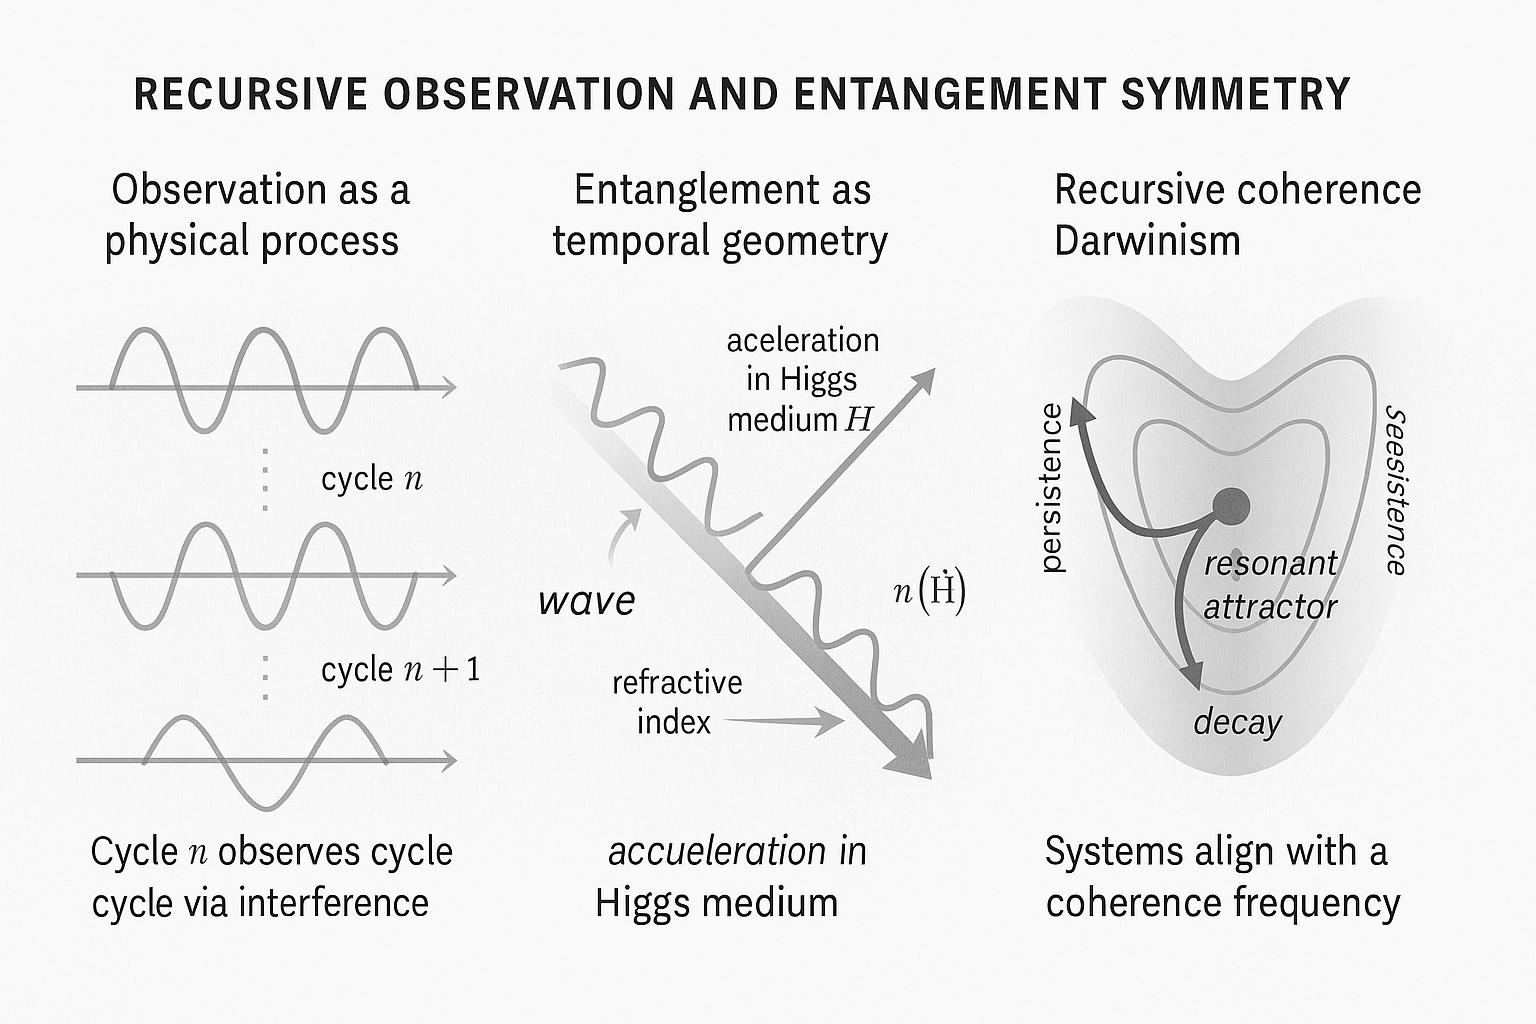
\includegraphics[width=0.75\textwidth]{figures/structural_time_dilation.png}
\caption{Structural time dilation: As a wavepacket accelerates through the Higgs field, its internal coherence structure deforms. The refractive index increases with field density, leading to wave flattening and decoherence—interpreted as the emergence of observed time.}
\label{fig:structural-time}
\end{figure}

\subsection*{7.3 Black Holes, Memory Collapse, and Reboot Conditions}

When recursive coherence fails, the system collapses. Black holes represent this condition cosmologically: entropy sinks where quantum memory vanishes. Their interiors exceed curvature bounds, and their holographic entropy saturates, triggering reboot. Supernovae, by contrast, emit coherent gravitational waves, acting as literal sources of recursive structure reinitialization.

We define reboot conditions formally as:
\begin{enumerate}
  \item Entropy threshold violation: \( S_n > S_{\text{max}}(E,n) \)
  \item Curvature singularity: \( R > R_{\text{crit}} \)
  \item Memory failure: \( \langle \Psi_n | \Psi_{n+1} \rangle \rightarrow 0 \)
\end{enumerate}

These boundaries correspond to the transition kernel’s failure to overlap with a coherent configuration, collapsing \( K(\phi, \phi') \) to a sharp peak with no forward propagation. This is the cosmological analog of wavefunction collapse~\cite{zurek_pointer_1981}.

\subsection*{7.4 Recursive Coherence Darwinism}

We define the governing principle of long-term survival in this model as:

\begin{quote}
\textbf{Recursive Coherence Darwinism:} Cycles tend toward a coherence frequency. Those that remain in phase persist. Those that deviate collapse.
\end{quote}

Convergence is favored through a coherence fitness functional \( \mathcal{F}_n \) (Appendix~C), which balances purity, entropy minimization, and recursive fidelity. Systems near the convergence field \( \mathcal{C}^*(\phi) \) are stabilized by Lyapunov dynamics. However, perfect alignment halts time: the system must either self-mutate or reset via reboot conditions.

This mirrors attractor dynamics in dynamical systems—feedback convergence under recursive memory constraints~\cite{tegmark_mathematical_2008,darwinism_cosmology_2018}.

\subsection*{7.5 Emotional and Physical Feedback Equivalence}

Gravitational waves encode not only mass-energy but coherence. Supernovae—violent, structured emissions—are literal astrophysical sources of both gravitational waves and recursive memory propagation. We conjecture that \textit{emotional singularities}, defined as extreme coherence collapse or resonance in conscious systems, are structurally equivalent.

Both initiate recursive redirection. Both act as memory emitters or sinks. The observer entanglement tensor \( O \), treated as an evolving internal field, encodes this feedback. It modulates the transition kernel, influences \( \Delta \theta \), and determines whether recursive propagation is sustained or halted.

The recursive universe is thus not indifferent—it is interactive. Structure feeds back. Emotion and gravity are dual expressions of the same coherence principle: \textbf{constructively interfere, or collapse}.

\vspace{1em}
\textit{“There are no observers outside the universe.”}~\cite{hartle_observation_2007}

\begin{figure}[H]
\centering
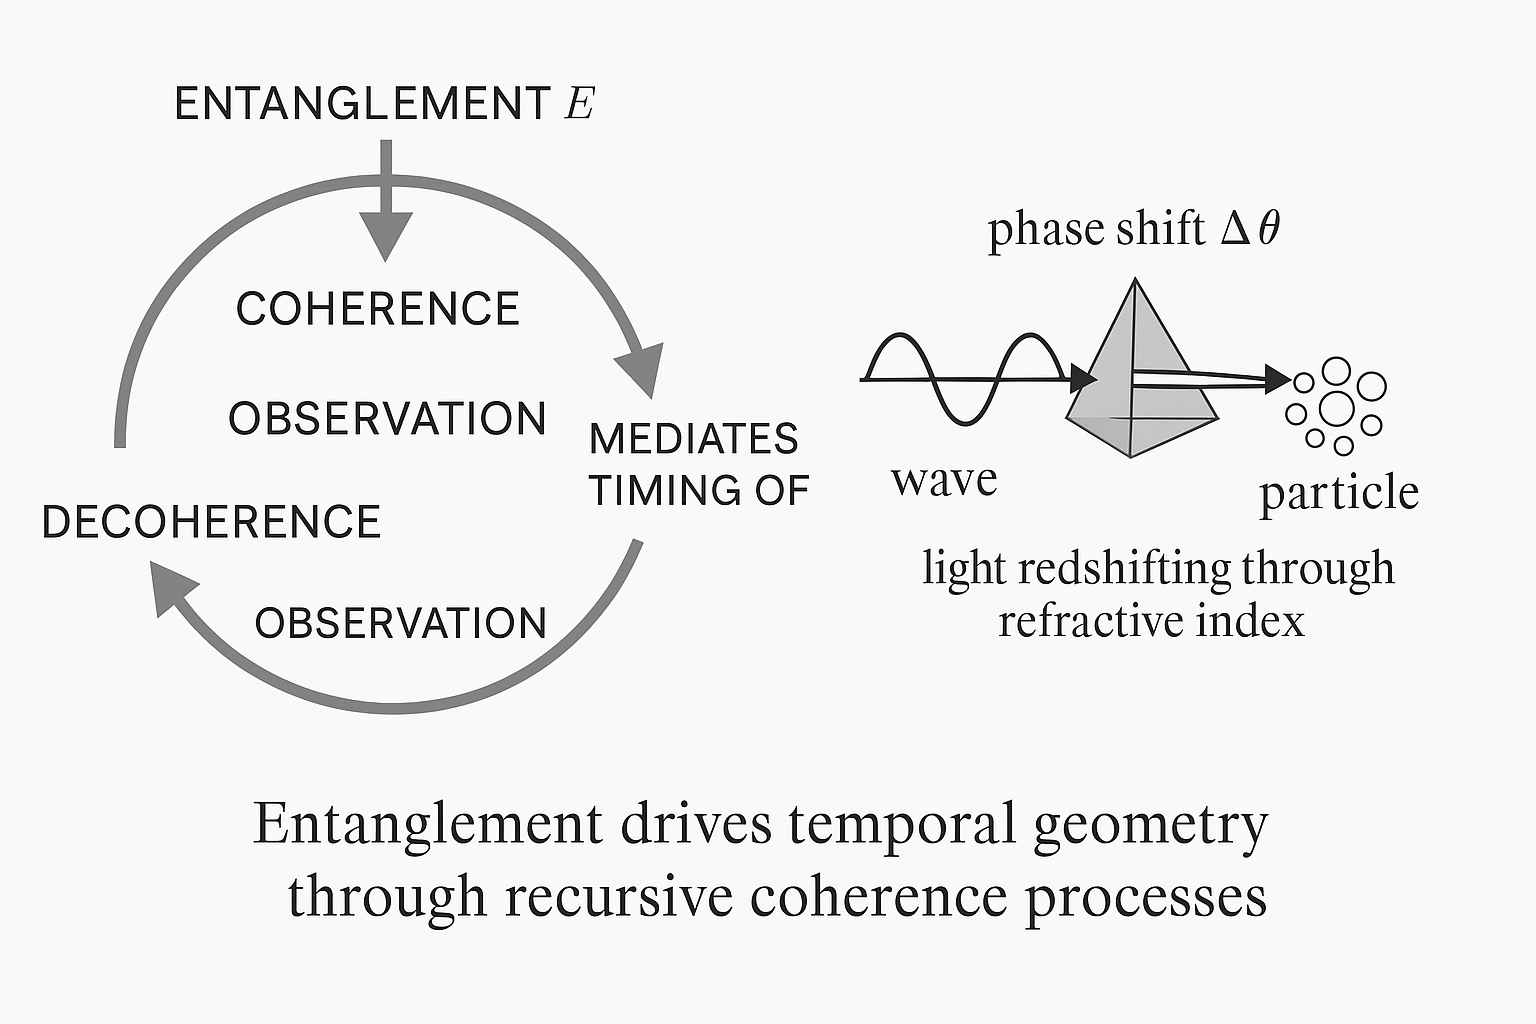
\includegraphics[width=0.75\textwidth]{figures/emotional_gravitational_feedback.png}
\caption{Dual feedback system. Gravitational wave emission (e.g., from supernovae) and emotional coherence collapse (e.g., psychological singularities) both trigger recursive redirection. The entanglement tensor \( O \) mediates feedback into the kernel, ensuring coherence or initiating reboot.}
\label{fig:feedback-equivalence}
\end{figure}

